\section{Deployment Results}
\label{sec:results}
\label{sec:results-anchor}
\InputIfFileExists{generated/results_status.tex}{}{}

\subsection{Artifact status and closed-loop reliability}
At the time of writing, \ValidRunCount{} of the \ExpectedRunCount{} planned primary runs are
available. They cover \AvailableScenarioCount{} traffic scenario(s) and
\AvailableSeedCount{} distinct seed(s). Failed and superseded runs are excluded by manifest
status and data quality before any database is opened: the pilot's exclusion list contains
exactly one entry, an earlier \texttt{ddpg\_only} seed-1 attempt that did not reach
\texttt{status=complete}. Two integrity caveats belong with these counts. First, the selector
keys candidate runs on the (scenario, arm, seed) triple and keeps the newest one; it does not
read the manifest \texttt{mode} field, so a frozen-policy re-evaluation run --- which validates
against a reduced phase set and can legitimately be marked complete and primary --- would
supersede the training run of the same cell. Such runs must be written to a separate results
directory until the selector filters on \texttt{mode}. Second, the raw evidence for this pilot
no longer exists. The three per-run SQLite databases ($\approx$1.3~GB each) and the trained
checkpoints were written to a results directory under \texttt{/tmp}; the testbed host was
subsequently rebooted to repair an NVIDIA driver/library version mismatch, and \texttt{/tmp} is
cleared on reboot, so those databases and checkpoints are permanently lost. What survives is
the derived artifact committed under \texttt{generated/}: \texttt{run\_metrics.csv} (213
columns, one row per selected run), \texttt{selected\_runs.csv}, the generated \LaTeX{} tables,
the three figures, and \texttt{artifact\_manifest.json}, which records the specification
SHA-256 and the OAI and FlexRIC revisions. Every number reported below therefore remains
traceable to a committed CSV column, but none of them can be re-derived from raw data and
\texttt{make results} can no longer regenerate the artifact. The campaign runs must archive
their databases on a persistent path rather than under \texttt{/tmp}.

\IfFileExists{generated/control_table.tex}{\begin{table*}[t]
\centering
\caption{Balanced seed-1 control-path and asynchronous learner reliability.}
\label{tab:pilot-control}
\begin{tabular}{lrrrrrr}
\toprule
Arm & Apply success (\%) & RC p99 (ms) & Tick p99 (ms) & Stale skip (\%) & Learner updates & Accepted Actors\\
\midrule
LLM-guided TD3 & 100.00 & 2.80 & 107.02 & 1.19 & 30207 & 62 \\
LLM only & 100.00 & 3.10 & 66.87 & 0.39 & 0 & 0 \\
TD3 only & 100.00 & 2.87 & 93.38 & 1.00 & 30266 & 257 \\
\bottomrule
\end{tabular}
\end{table*}
}{No generated control table is available.}

As Table~\ref{tab:pilot-control} records, all three selected runs reported 100\% five-UE
coverage over their own transition window and received an E2 acknowledgement for every
recorded control (apply success 100\%). The
persistent actuator kept RC control latency in the low-millisecond range, with a p99 of
2.80--3.10~ms against the 20~ms bound. Controller tick jitter p99 was 66.87--107.02~ms against
the 150~ms bound, and the stale-state skip rate was 0.39--1.19\% against the 50\% bound. The
measured fresh-state action interval averaged 101.3--103.6~ms, slightly above the nominal
100~ms clock, because a tick that sees no newer 50~ms summary is skipped rather than
fabricating a transition; its p95 was 166~ms for all three arms, inside the enforced 180~ms
bound, while the p99 of 208--231~ms is recorded but not gated.
\FloatBarrier

\subsection{Intent satisfaction and throughput}
Throughout this section, \emph{SLA satisfaction} is the fraction of control steps in which the
protected slice met its calibrated floor, and \emph{intent satisfaction} is the strictly
stronger condition that the SLA holds \emph{and} the commanded PRB share of the priority slice
is at least the configured minimum of 55\%. Throughput figures are RLC-derived aggregates from
the near-RT state, not iperf receiver goodput.

\ifFullCampaign
\IfFileExists{generated/campaign_table.tex}{\begin{table*}[t]
\centering
\caption{Complete-campaign scenario means. Statistical comparisons use paired seeds rather than these unpaired row means.}
\label{tab:campaign-performance}
\begin{tabular}{llrrrrr}
\toprule
Scenario & Arm & Seeds & I1 satisfaction (\%) & I2 satisfaction (\%) & I1 total TH & I2 total TH\\
\midrule
balanced & LLM-guided TD3 & 1 & 100.00 & 99.94 & 97.35 & 96.44 \\
balanced & LLM only & 1 & 99.94 & 99.39 & 94.58 & 92.14 \\
balanced & TD3 only & 1 & 79.94 & 69.78 & 95.49 & 93.73 \\
\bottomrule
\end{tabular}
\end{table*}
}{No generated campaign table is available.}
\IfFileExists{generated/paired_table.tex}{\begin{table*}[t]
\centering
\caption{Same-seed paired bootstrap comparisons. Positive values favor guided control.}
\label{tab:paired-results}
\begin{tabular}{lllrrl}
\toprule
Scenario & Comparison & Metric & Pairs & Mean difference & 95\% CI\\
\midrule
balanced & Guided $-$ TD3 only & Intent satisfaction & 1 & 0.251 & [0.251, 0.251] \\
balanced & Guided $-$ TD3 only & Total DL TH & 1 & 2.277 & [2.277, 2.277] \\
balanced & Guided $-$ LLM only & Intent satisfaction & 1 & 0.003 & [0.003, 0.003] \\
balanced & Guided $-$ LLM only & Total DL TH & 1 & 3.536 & [3.536, 3.536] \\
\bottomrule
\end{tabular}
\end{table*}
}{}
The complete campaign is analyzed per scenario with same-seed pairing in
Table~\ref{tab:campaign-performance} and Fig.~\ref{fig:pilot-performance}; cross-scenario values are equal-weight macro averages rather than pooled windows.
\else
The available data constitute a balanced-load seed-1 pilot.
\IfFileExists{generated/performance_table.tex}{\begin{table*}[t]
\centering
\caption{Balanced seed-1 pilot. Satisfaction is the fraction of frozen evaluation windows meeting the active intent. Throughput values are RLC-derived Mbps.}
\label{tab:pilot-performance}
\begin{tabular}{lrrrrrr}
\toprule
& \multicolumn{2}{c}{Intent satisfaction (\%)} & \multicolumn{2}{c}{Total DL TH} & \multicolumn{2}{c}{Protected p5 DL TH}\\
Arm & I1 & I2 & I1 & I2 & I1 & I2\\
\midrule
LLM-guided TD3 & 100.00 & 99.94 & 97.35 & 96.44 & 32.60 & 34.35 \\
LLM only & 99.94 & 99.39 & 94.58 & 92.14 & 31.19 & 31.02 \\
TD3 only & 79.94 & 69.78 & 95.49 & 93.73 & 25.69 & 33.50 \\
\bottomrule
\end{tabular}
\end{table*}
}{No generated performance table is available.}

As Table~\ref{tab:pilot-performance} and Fig.~\ref{fig:pilot-performance} report, guided
control attained 100.00\% and 99.94\% intent satisfaction for the two intent directions
and delivered 97.35 and 96.44~Mbps aggregate downlink throughput. Relative to unguided
learning this is $+20.06$ and $+30.17$ percentage points of intent satisfaction. Relative to
LLM-only it is $+2.77$ and $+4.30$~Mbps of aggregate throughput (94.58 and 92.14~Mbps), with
protected-slice 5th-percentile throughput at least as high in both directions (32.60 and
34.35~Mbps versus 31.19 and 31.02~Mbps). One comparison runs the other way: over the first 300
training transitions the LLM-only arm accumulated the highest reward of the three arms
(276.51, versus 261.43 for guided and 157.55 for unguided), which is unsurprising for a policy
that simply executes a projected teacher and never explores. These values support end-to-end
feasibility and motivate the paired campaign; they do not establish statistical superiority.

\IfFileExists{generated/guided_vs_ddpg_table.tex}{\begin{table*}[t]
\centering
\caption{Direct balanced seed-1 comparison with the unguided \texttt{ddpg\_only} arm. Percentage deltas are percentage-point differences. Lower is better for SLA violation, saturation, and TD error.}
\label{tab:guided-vs-ddpg}
\begin{tabular}{lrrr}
\toprule
Metric & LLM-guided TD3 & DDPG-only (TD3-style) & Guided $-$ DDPG-only\\
\midrule
Intent 1 satisfaction (\%) & 100.00 & 79.94 & +20.06 \\
Intent 2 satisfaction (\%) & 99.94 & 69.78 & +30.17 \\
Early SLA violation (\%) & 0.00 & 12.00 & -12.00 \\
Early reward AUC & 261.43 & 157.55 & +103.87 \\
Intent 1 total DL TH (Mbps) & 97.35 & 95.49 & +1.85 \\
Intent 2 total DL TH (Mbps) & 96.44 & 93.73 & +2.70 \\
Intent 1 protected p5 TH (Mbps) & 32.60 & 25.69 & +6.92 \\
Intent 2 protected p5 TH (Mbps) & 34.35 & 33.50 & +0.85 \\
Training Actor saturation (\%) & 14.74 & 0.40 & +14.34 \\
Learner mean TD error & 0.0830 & 0.0558 & +0.0272 \\
\bottomrule
\end{tabular}
\end{table*}
}{}

The direct DDPG-only comparison in Table~\ref{tab:guided-vs-ddpg} separates guidance gains from
LLM-only behavior. During the
first 300 training transitions, guided control had no SLA violations and no intent violations,
compared with 12.00\% and 50.67\%\footnote{The 50.67\% value is the training-phase
first-300-transition metric, recorded as
\texttt{training\_early\_intent\_violation\_rate} in \texttt{generated/run\_metrics.csv}. The
generator's top-level \texttt{early\_intent\_violation\_rate} column of the same file instead
carries the Intent-1 evaluation value (17.67\%) and must not be read as the training-phase
quantity.} for DDPG-only, and its reward over that window was 65.9\%
higher (261.43 versus 157.55). Over the whole training phase the unguided arm accumulated an
SLA deficit area of 43.93 against 0.92 for guided control. In frozen evaluation, guidance
increased aggregate throughput by 1.94\% and 2.88\% for the two intent directions. The largest
reliability difference occurred for Intent~1, where protected-slice p5 throughput increased
from 25.69 to 32.60~Mbps; for Intent~2 the same quantity moved only from 33.50 to
34.35~Mbps, so the reliability benefit was direction-dependent rather than uniform.

The result is not uniformly favorable to guidance. Guided training had a 14.74\% Actor
saturation rate and a mean learner TD error of 0.0830, versus 0.40\% and 0.0558 for DDPG-only.
The clearer signature, however, is the acknowledged-action boundary rate: 90.66\% of guided
training actions and 92.11\%/78.22\% of its two evaluation phases sat within half a PRB of an
edge of the active feasible interval, against 0.34\%/0.00\%/0.00\% for the unguided arm. The
mechanism is visible in the allocations themselves. With a 55\% minimum priority ratio the
guided Intent-1 feasible interval starts at $b_A=59$ of 106 PRBs and the guided Intent-1 mean
was 59.27 PRBs; symmetrically the Intent-2 interval ends at $b_A=47$ and the guided mean was
46.67 PRBs. Action-bin coverage in evaluation fell to 0.8 for guided control while DDPG-only
reached 1.0 and 0.9. Guided control therefore operated essentially on its guidance boundary
rather than searching inside it, placing it between the unguided learner and the LLM-only arm,
whose boundary rate was 89.28--100\% at a bin coverage of 0.1. The pilot thus supports
guidance as a safety and task-alignment mechanism while showing that, as configured here, the
constrained action region and teacher influence substantially reduce policy diversity.
\fi
\FloatBarrier

\subsection{DDPG-only baseline behavior}
\IfFileExists{generated/ddpg_only_phase_table.tex}{\begin{table*}[t]
\centering
\caption{DDPG-only phase behavior. Slice-A ratio is the acknowledged command for S-NSSAI \texttt{1:ffffff}; full intent satisfaction requires both the protected-slice floor and the active priority-ratio condition.}
\label{tab:ddpg-only-phases}
\begin{tabular}{llrlrrrr}
\toprule
Scenario & Runs & Phase & Steps & Reward & SLA sat. (\%) & Intent sat. (\%) & Slice-A ratio (\%)\\
\midrule
balanced & 1 & Calibration & 1000 & 1.367 & 100.00 & 100.00 & 50.00 \\
balanced & 1 & Training & 36000 & 0.797 & 98.84 & 66.44 & 52.46 \\
balanced & 1 & Intent 1 evaluation & 1800 & 0.862 & 98.78 & 79.94 & 60.40 \\
balanced & 1 & Intent 2 evaluation & 1800 & 0.867 & 99.83 & 69.78 & 44.29 \\
\bottomrule
\end{tabular}
\end{table*}
}{No generated DDPG-only phase table is available.}

\IfFileExists{generated/ddpg_only_priority_table.tex}{\begin{table*}[t]
\centering
\caption{DDPG-only training behavior by priority direction. Throughput is RLC-derived Mbps. The minimum priority ratio is part of the machine-readable intent objective, not the protected-slice throughput SLA.}
\label{tab:ddpg-only-priority}
\begin{tabular}{llrrrrrrr}
\toprule
Scenario & Runs & Priority slice & Action (\%) & Required (\%) & Priority TH & Protected TH & SLA sat. (\%) & Intent sat. (\%)\\
\midrule
balanced & 1 & 1:123456 & 54.80 & 55.00 & 48.97 & 41.82 & 99.38 & 56.29 \\
balanced & 1 & 1:ffffff & 59.71 & 55.00 & 55.58 & 36.36 & 98.30 & 76.59 \\
\bottomrule
\end{tabular}
\end{table*}
}{}

\ifFullCampaign
Tables~\ref{tab:ddpg-only-phases} and~\ref{tab:ddpg-only-priority} and Fig.~\ref{fig:ddpg-only-learning} report per-scenario means across independently trained seeds. They are descriptive diagnostics; same-seed policy comparisons remain in Table~\ref{tab:paired-results}.
\else
The calibration row of Table~\ref{tab:ddpg-only-phases} is not a policy measurement and is not
comparable with the other rows. Calibration runs under a permissive bootstrap intent that
carries a 10~Mbps placeholder floor and publishes no policy constraints, so the priority-ratio
term of the intent test is inert and the floor is trivially met; its 50.00\% mean Slice-A
share is simply the arithmetic mean of the fixed sweep $\{25,35,50,65,75\}$, and its reward of
1.367 is computed under that permissive objective.

The DDPG-only pilot completed 36{,}000 training control steps and 30{,}266 asynchronous
learner updates. It satisfied the protected-slice throughput floor in 98.84\% of training
transitions but met the complete intent in only 66.44\%. This difference is expected from the
implemented objective: SLA satisfaction checks the protected throughput floor, whereas
complete intent satisfaction additionally requires the commanded priority slice to receive at
least 55\% of PRBs.

The learned policy changed direction with the intent, as the binned training curves of
Fig.~\ref{fig:ddpg-only-learning} show. In frozen evaluation, the Slice-A
command averaged 60.40\% when Slice~A was prioritized and 44.29\% when Slice~B was
prioritized, with intent satisfaction of 79.94\% and 69.78\% respectively. Over the 18{,}000
training transitions of each direction, the \snssaiA-priority direction attained 76.6\% intent
satisfaction against 56.3\% for \snssaiB-priority. The priority-direction table shows why: in
the \snssaiB-priority direction the mean commanded share of the priority slice was 54.80\%,
just below the 55\% requirement, so a small systematic bias in the commanded allocation
converts directly into a large intent-satisfaction loss even though SLA satisfaction stayed at
99.38\%. This asymmetry is consistent with the balanced per-UE load yielding unequal aggregate
demands: three Slice-A UEs offer 90~Mbps while two Slice-B UEs offer 60~Mbps.

The DDPG-only Actor did not collapse to an action-space boundary. Its training saturation rate
was 0.40\%, its acknowledged-action boundary rate was 0.34\%, all ten action bins were visited
during training, and its mean learner TD error was 0.0558. The pilot therefore indicates
directional learning with broad action-space coverage, but not a policy that robustly
satisfies both intent directions: its training SLA deficit area of 43.93 is roughly 48 times
that of guided control. The guided advantage in this run is principally lower cold-start
violation and stronger task alignment, rather than recovery from unguided boundary collapse.
\fi

\begin{figure*}[t]
  \centering
  \IfFileExists{generated/balanced_ddpg_only_diagnostics.png}{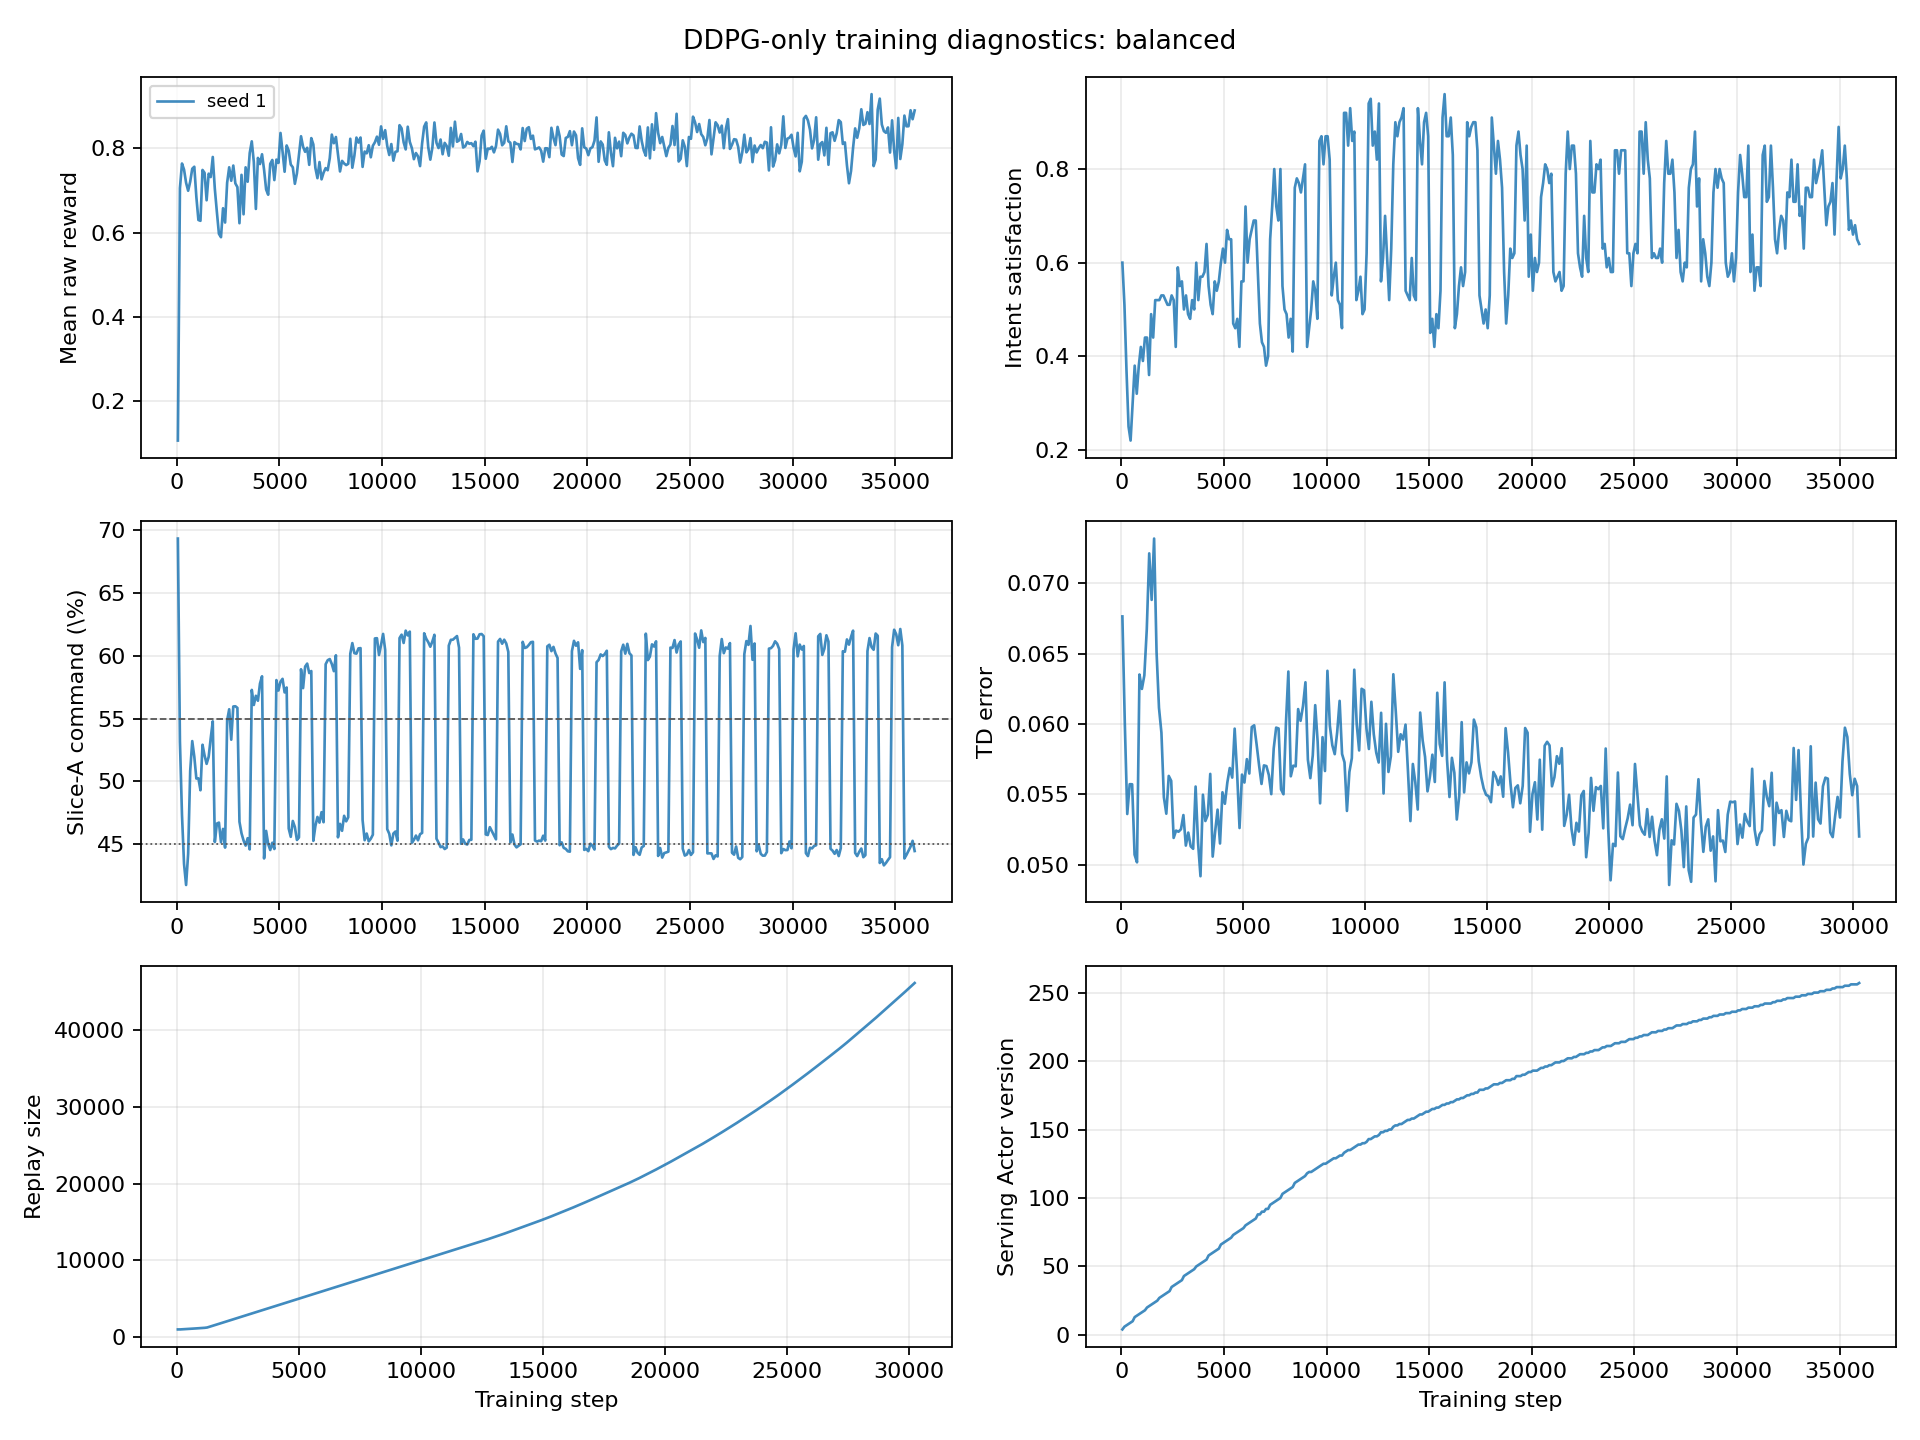
\includegraphics[width=0.94\textwidth]{generated/balanced_ddpg_only_diagnostics.png}}{\fbox{Generate results to create the DDPG-only diagnostics.}}
  \caption{DDPG-only training diagnostics. Curves are aggregated into 100-transition bins; the single-seed pilot is shown without a confidence envelope. The two dashed Slice-A levels indicate the 55\% A-priority and equivalent 45\% B-priority command thresholds.}
  \label{fig:ddpg-only-learning}
\end{figure*}

\begin{figure}[t]
  \centering
  \IfFileExists{generated/balanced_performance_comparison.png}{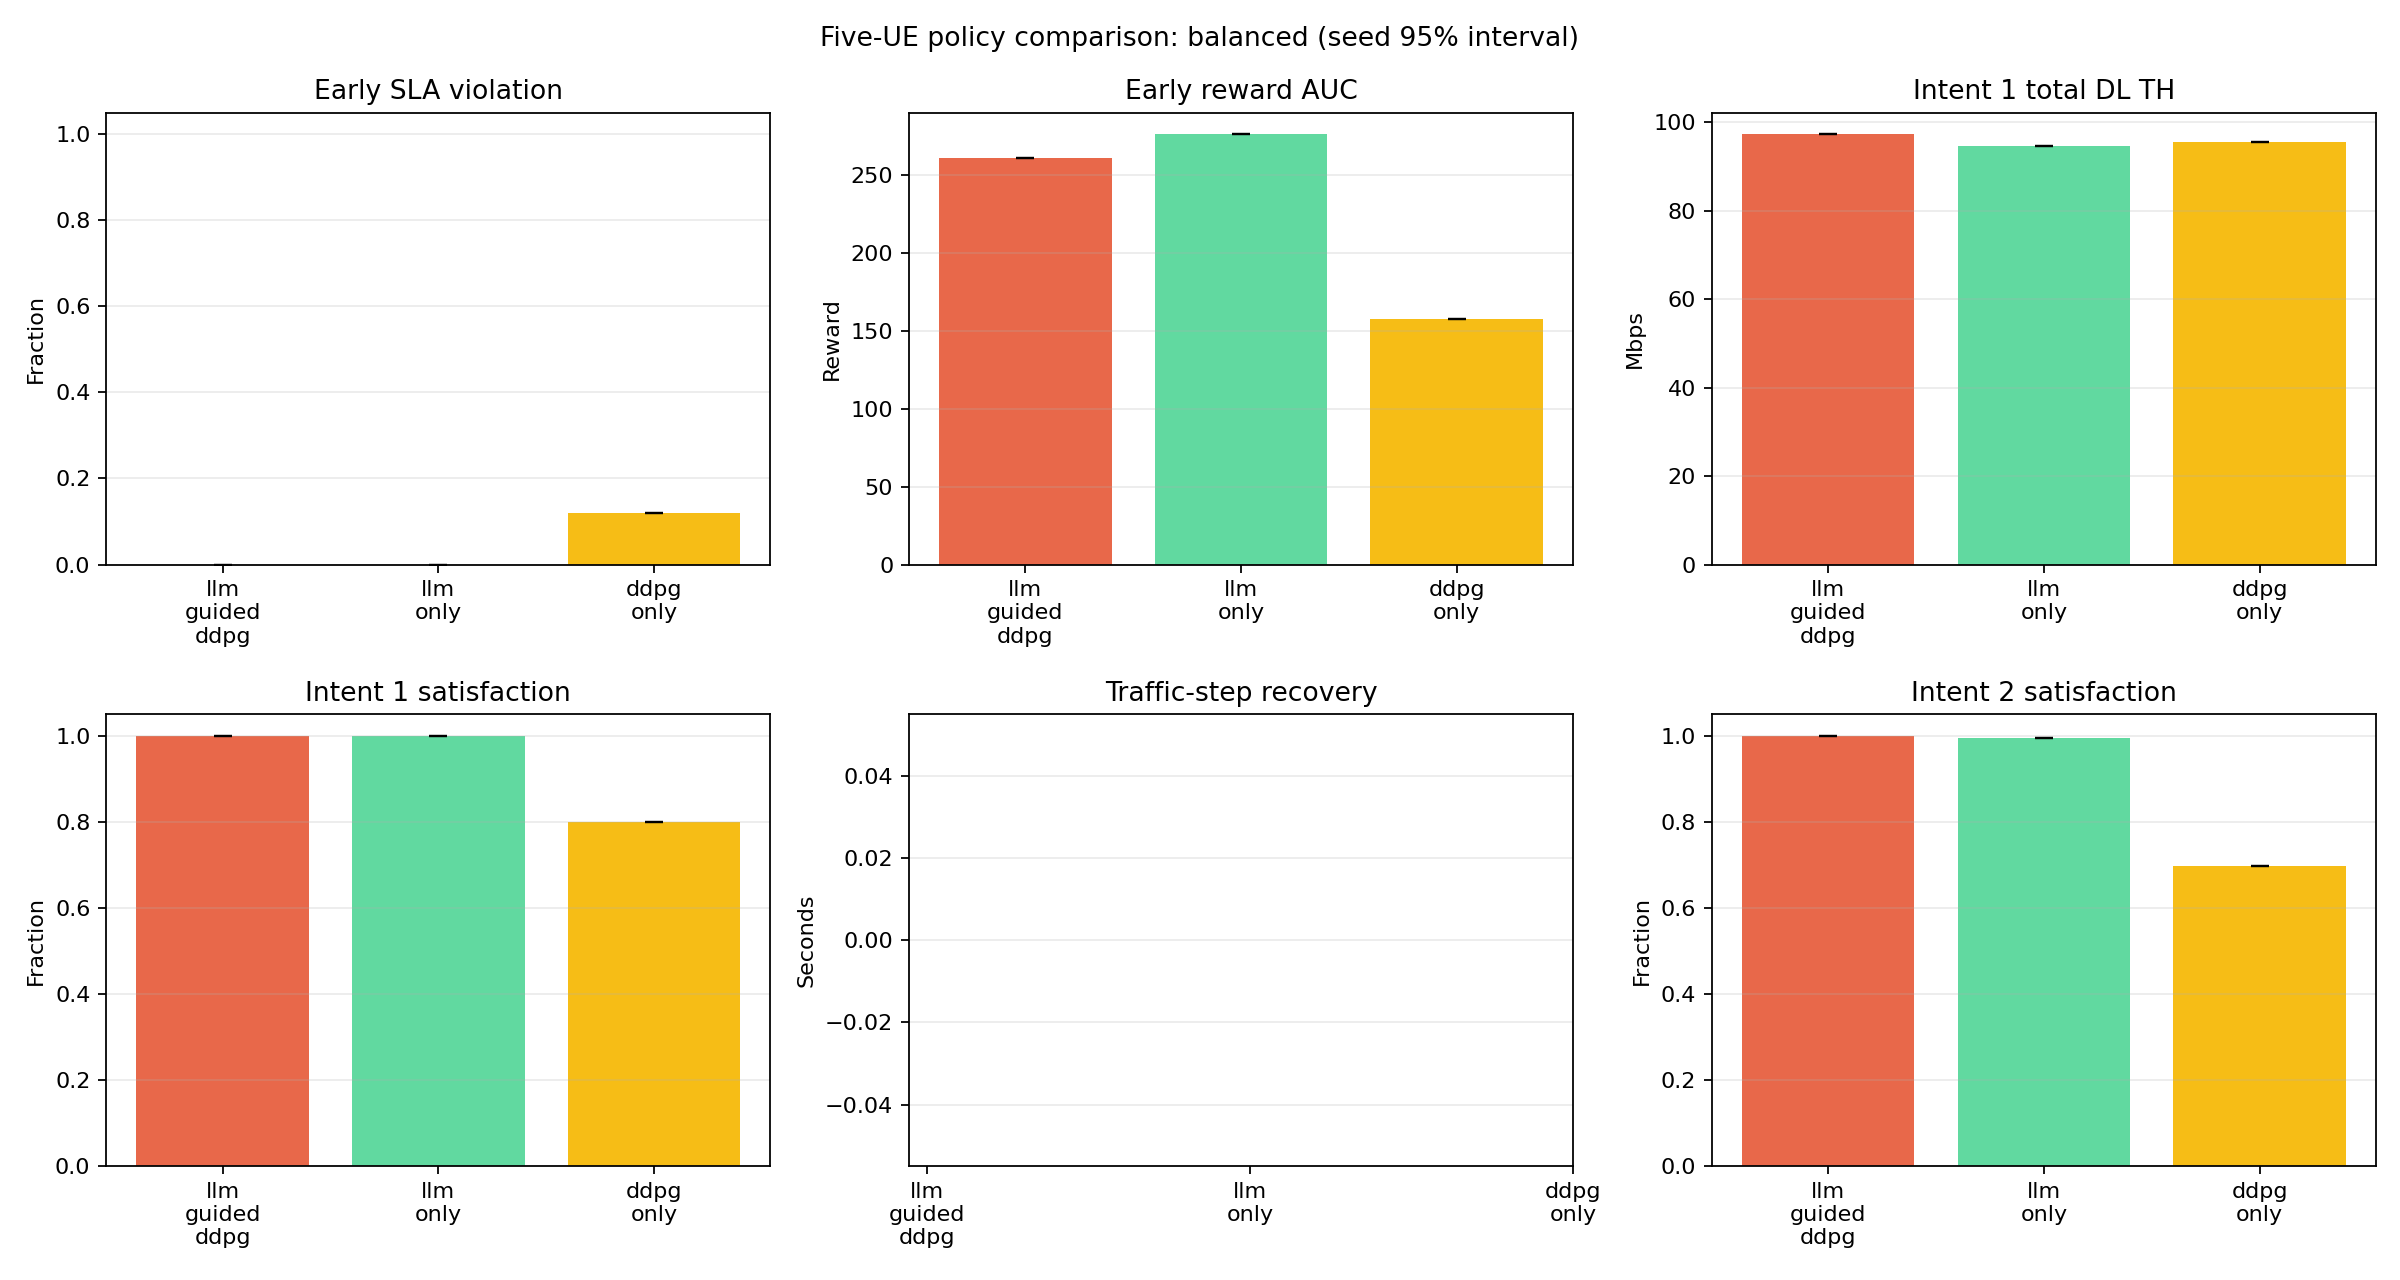
\includegraphics[width=\columnwidth]{generated/balanced_performance_comparison.png}}{\fbox{Generate results to create this figure.}}
  \caption{Balanced seed-1 performance comparison. Confidence intervals are intentionally omitted for the single-seed pilot.}
  \label{fig:pilot-performance}
\end{figure}
\FloatBarrier

\subsection{Learning behavior}
Each learning arm logged the full 40{,}600 protocol control steps of the four validated phases
and inserted about $4.6\times10^4$ transitions into the asynchronous replay --- 45{,}726 for
guided control and 46{,}317 for the unguided arm --- the surplus over the 1{,}000 prefilled
calibration and 36{,}000 training transitions being uncounted intent-switch steps. Every
inserted transition passed the per-transition trainability test in every phase. The learner
performed 30{,}207 and 30{,}266 updates at 6.57 and 6.54~Hz, of which 15{,}103 and 15{,}133
were Actor updates because of the delayed-update interval of two. Replay rows reached the
learner with a mean insertion age of 1.74~s (guided) and 1.65~s (unguided) at mean queue
depths of about 2{,}900 and 3{,}000 rows, which quantifies the decoupling between the 100~ms
control loop and the learner; Fig.~\ref{fig:learning} plots the resulting learner diagnostics.

Candidate publication behavior differed sharply. Both learning arms produced 257 candidate
Actors, but the guided run accepted 62 and rejected 195, whereas the unguided run accepted all
257. The accepted count for the guided run is an upper bound on genuine quality-gate passes:
the learner implements a force-promotion escape hatch that publishes a gate-failing candidate
after six consecutive rejections, provided it is finite and projects legally into the active
bounds, and the per-candidate accepted/forced split was recorded only in the run databases,
which are lost, so the split cannot now be recovered for this pilot. The
serving path diverged further from the candidate stream: the controller observed 61 distinct
serving Actor versions and performed 50 atomic swaps in the guided run, against 244 versions
and 204 swaps in the unguided run, with a maximum swap cost below 0.7~ms in both. The
distinction between candidate records, accepted versions, and actually served versions is
preserved in the artifact.

\begin{figure}[t]
  \centering
  \IfFileExists{generated/balanced_ddpg_learning.png}{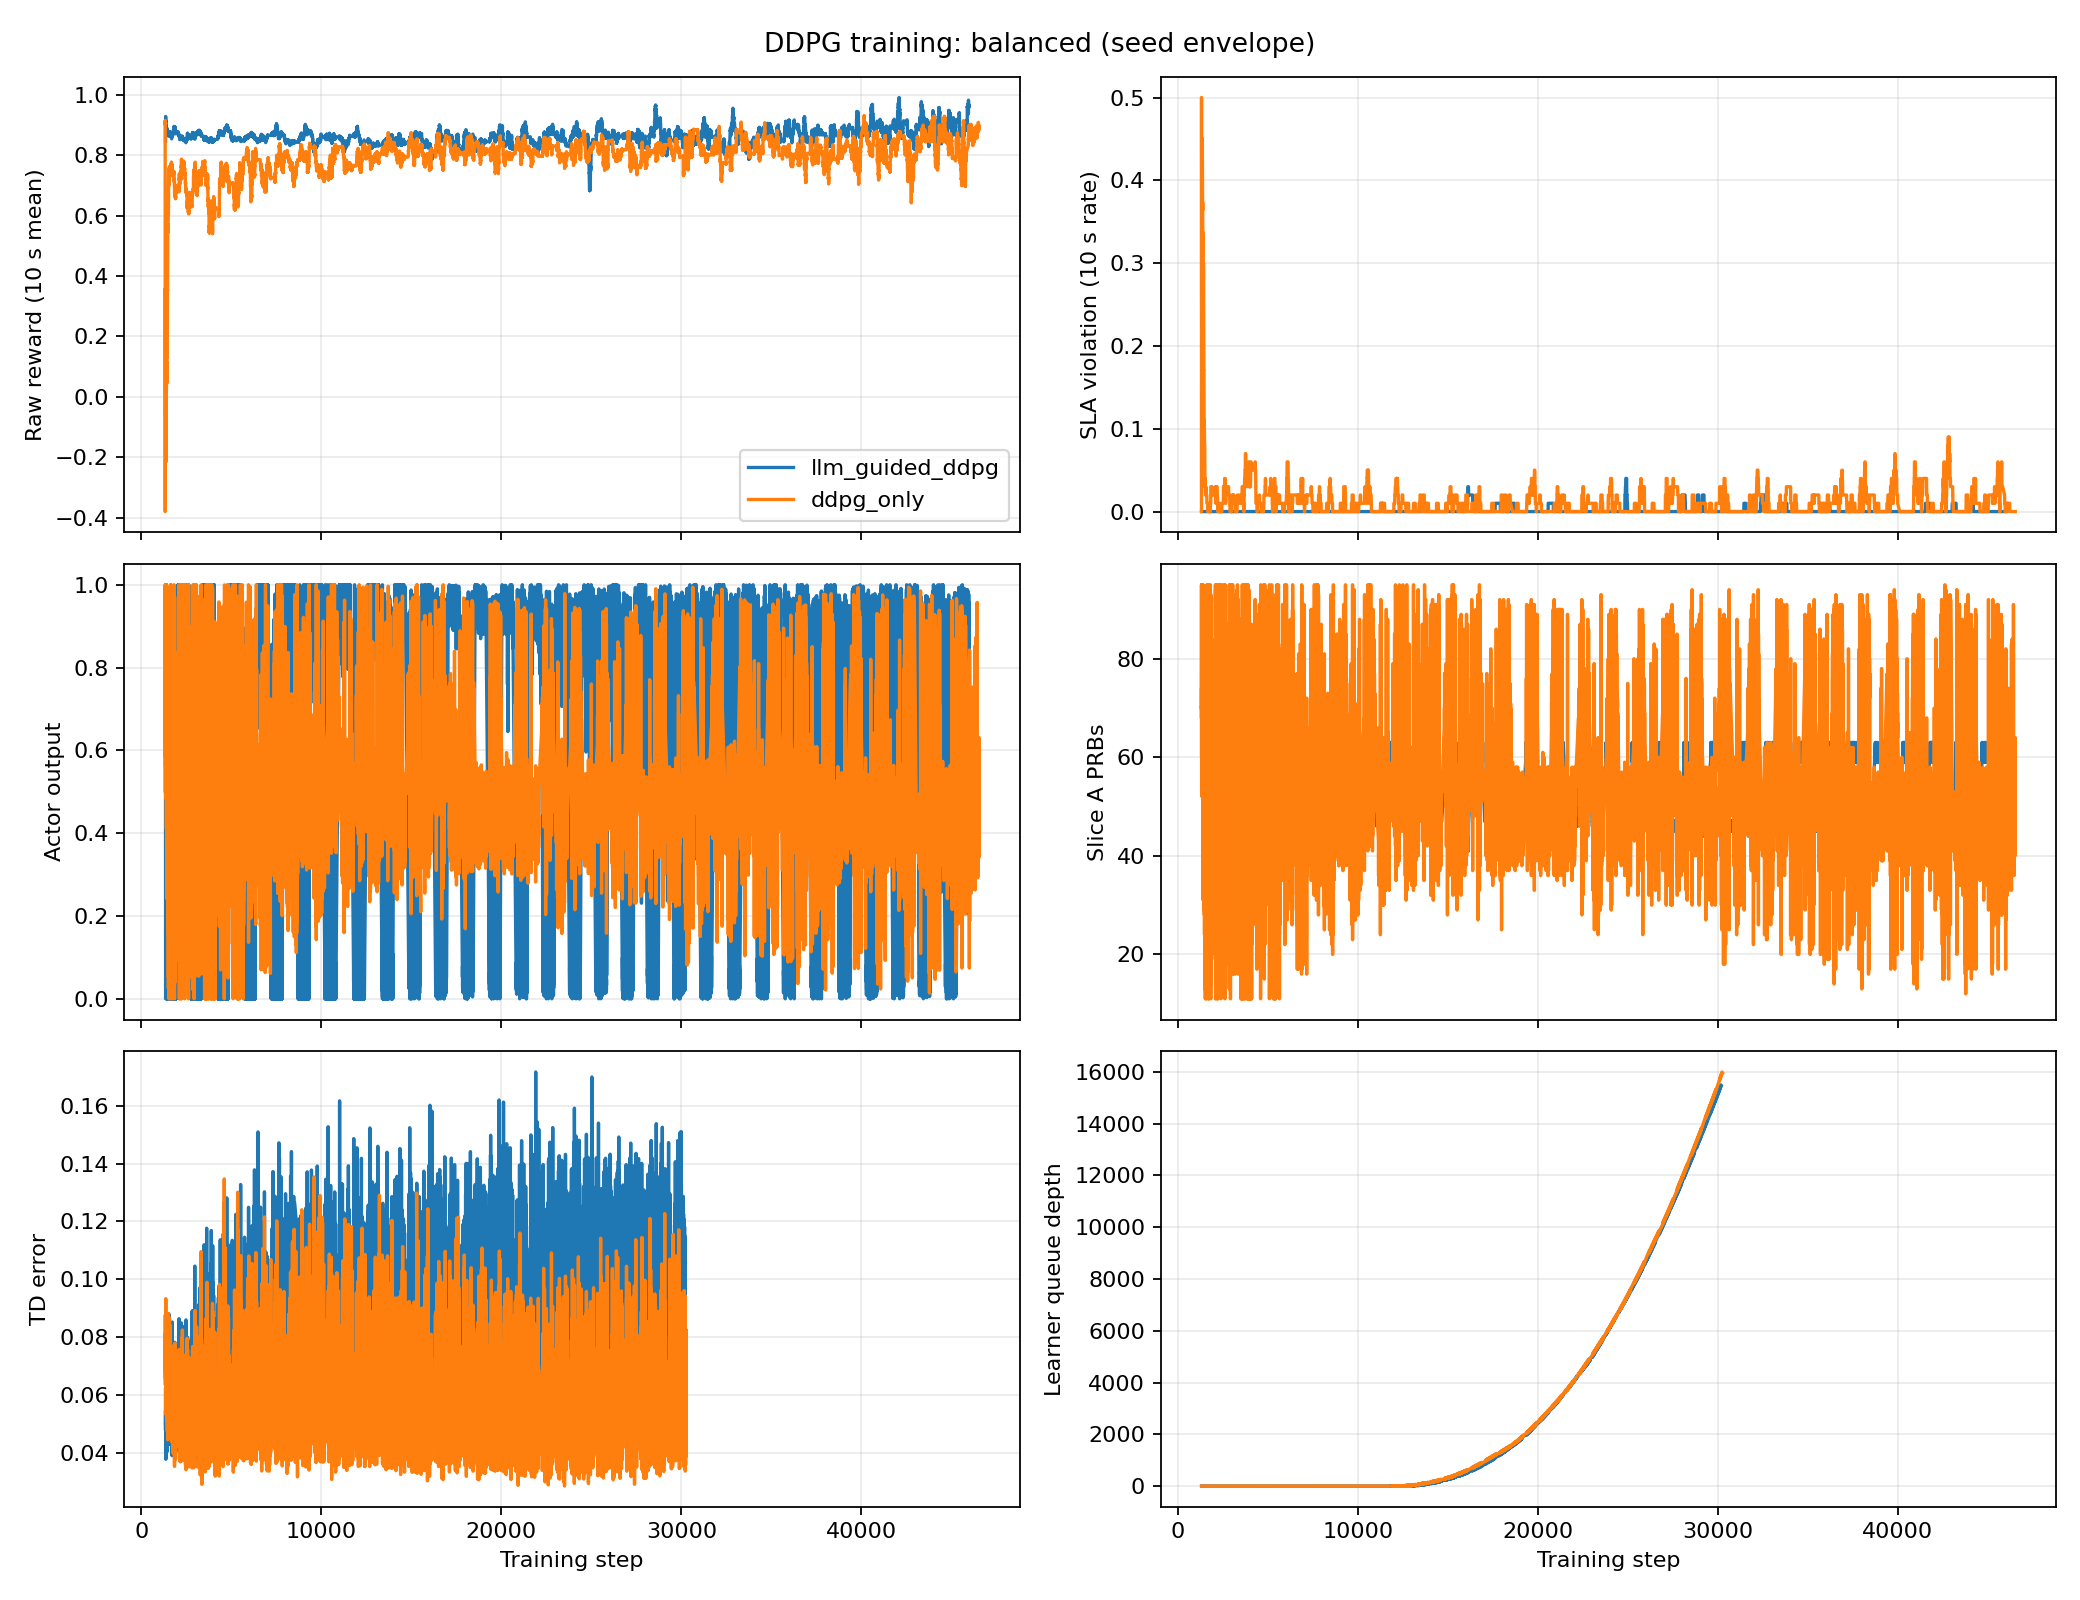
\includegraphics[width=\columnwidth]{generated/balanced_ddpg_learning.png}}{\fbox{Generate results to create this figure.}}
  \caption{Learning diagnostics generated from raw experiment and learner tables.}
  \label{fig:learning}
\end{figure}

The UDP offered load intentionally saturates the radio. Against 30~Mbps offered per UE, the
mean delivered rate at the UE TUN interface was 17.8--18.4~Mbps, i.e.\ 38.8--40.5\%
offered-versus-delivered downlink loss across the three arms. This figure is computed from
receiver byte counters against the nominal offered rate; it is not the iperf3 sender's own
datagram-loss report, and it is therefore not a control failure but the expected consequence
of running the cell in overload so that the PRB ratio is the binding constraint. We
consequently keep receiver goodput and RLC-derived throughput as separate quantities
throughout. All three arms recorded the same traffic trace hash, confirming that they were
offered identical load. The dynamic heavy-load scenarios, in which the 5~s phase pattern is
imposed by the HTB shaper of Section~\ref{sec:methodology}, are
required to assess response to demand shifts and remain placeholders until complete primary
runs are available; because the balanced pilot never installs the shaper, its 100\% segment
success rate carries no information about shaper fidelity.

\ifFullCampaign\else
The full 3-scenario, 3-arm, 5-seed campaign is incomplete. No paired-bootstrap interval or
cross-scenario claim is reported in this version, and no statement in this section should be
read as a statistical comparison: every value above comes from one seed of one scenario.
\fi
\FloatBarrier
